% A skeleton file for producing Computer Engineering reports
% https://kgcoe-git.rit.edu/jgm6496/KGCOEReport_template

\documentclass[CMPE]{../KGCOEReport}

% The following should be changed to represent your personal information
\newcommand{\classCode}{CMPE 260}  % 4 char code with number
\newcommand{\name}{Andrei Tumbar}
\newcommand{\LabSectionNum}{1}
\newcommand{\LabInstructor}{Moskal}    % The slash is to tell LaTeX that the period is between words
% not sentences so it spaces correctly. It won't appear in the
% final pdf
\newcommand{\TAs}{Jacob Meyerson\\Dennis Lam}
\newcommand{\LectureSectionNum}{1}
\newcommand{\LectureInstructor}{Cliver}
\newcommand{\exerciseNumber}{5}
\newcommand{\exerciseDescription}{Memory \& Writeback Stage}
\newcommand{\dateDone}{March 30th}
\newcommand{\dateSubmitted}{April 17th}

\usepackage{tikz}
\usepackage{circuitikz}
\usetikzlibrary{calc}
\usetikzlibrary{circuits.logic.IEC,calc}
\usepackage{multirow}
\usepackage{float}
\usepackage{lmodern}
\usepackage{siunitx}
\usepackage{subcaption}
\usepackage{graphicx}
\usepackage[usestackEOL]{stackengine}
\usepackage{scalerel}
\usepackage[T1]{fontenc}
\usepackage{amsmath}

\def\lbar#1{\ThisStyle{%
    \setbox0=\hbox{$\SavedStyle#1$}%
    \stackengine{2.2\LMpt}{$\SavedStyle#1$}{\rule{\wd0}{0.1\LMpt}}{O}{c}{F}{F}{S}%
}}

\DeclareFontFamily{U}{mathx}{\hyphenchar\font45}
\DeclareFontShape{U}{mathx}{m}{n}{ <-> mathx10 }{}
\DeclareSymbolFont{mathx}{U}{mathx}{m}{n}
\DeclareFontSubstitution{U}{mathx}{m}{n}
\DeclareMathAccent{\widebar}{\mathalpha}{mathx}{"73}

\makeatletter
\newcommand{\cwidebar}[2][0]{{\mathpalette\@cwidebar{{#1}{#2}}}}
\newcommand{\@cwidebar}[2]{\@cwideb@r{#1}#2}
\newcommand{\@cwideb@r}[3]{%
    \sbox\z@{$\m@th\mkern-#2mu#3\mkern#2mu$}%
    \widebar{\box\z@}%
}
\newcommand\currentcoordinate{\the\tikz@lastxsaved,\the\tikz@lastysaved}
\makeatother

\newcommand\decbin[9]{%
    \par\smallskip
    \makebox[3cm][r]{$#1$\ }\fbox{#2}\,\fbox{#3}\,\fbox{#4}\,\fbox{#5}\,\fbox{#6}\,\fbox{#7}\,\fbox{#8}\,\fbox{#9}\par}


\def\code#1{\texttt{#1}}

\begin{document}
    \maketitle
    \section*{Abstract}

    In this laboratory exercise, the data memory, memory stage, and writeback
    stages of the MIPS datapath were implemented. The data memory was essentially
    equivalent to the instruction memory however it was written to be word
    addressable. This implementation initialized 1024 words in data memory.
    The writeback stage will simply select between the ALU output and the memory
    data output to write back to the register file.

    \section*{Design Methodology}

    The given Verilog implementation of memory stage 
    (bar the seven segment display, and switches) is very similar to 
    the design of the instruction memory. The only major difference that can 
    be seen is the addressablilty of data memory. Instead of concatenating 
    four consecutive bytes as done with the instruction memory, the data 
    memory will address by word meaning adjecent addresses will be 4-bytes apart.
    \\
    
    The Verilog implementation of the writeback stage is fairly straightforward.
    There are a series of passthrough signals which a simply copied or inverted
    to the outputs. The VHDL implementation of the writeback will differ slightly
    because the output signal \code{reg\_write} will be manually controlled by 
    an input signal instead of by the inverted \code{mem\_write} signal. Other than
    the passthrough signals, the writeback stage will control the writeback data
    output by selecting between the ALU result data and the memory read data to
    write back to the register file.
	
    \section*{Results \& Analysis}

	\subsection*{Memory Stage}

    To test the memory stage, a testbench was written to verify its functionality
    by sequentially writing and then reading from memory. An extra read cycle
    was added to verify that the first read cycle did not overwrite the memory
    at the target address.
    
    \begin{table}[H]
        \renewcommand{\arraystretch}{1.2}
        \setlength{\tabcolsep}{12pt}
        \caption{Memory Stage Testcases}
        \begin{center}
            \begin{tabular}{|c|c|c|}
                \hline
				Address & Operation & Value\\\hline

				%  address      Operation          Value     
				\code{0x1B} & \code{WRITE} & \code{0xAAAA5555}\\\hline
				\code{0x1C} & \code{WRITE} & \code{0x5555AAAA}\\\hline
				\code{0x1B} & \code{READ} & \code{0xAAAA5555}\\\hline
				\code{0x1C} & \code{READ} & \code{0x5555AAAA}\\\hline
				\code{0x1B} & \code{READ} & \code{0xAAAA5555}\\\hline
				\code{0x1C} & \code{READ} & \code{0x5555AAAA}\\\hline

            \end{tabular}
        \end{center}
        \label{tab:mem}
    \end{table}
    
    As shown in Table \ref{tab:mem}, the first two operations will write
    to two difference memory addresses. The next four operations will verify
    the values of these addresses by performing read operations.
    
    A set of waveforms was generated to show the simulation output.
    
    \begin{figure}[h!]
        \centering
        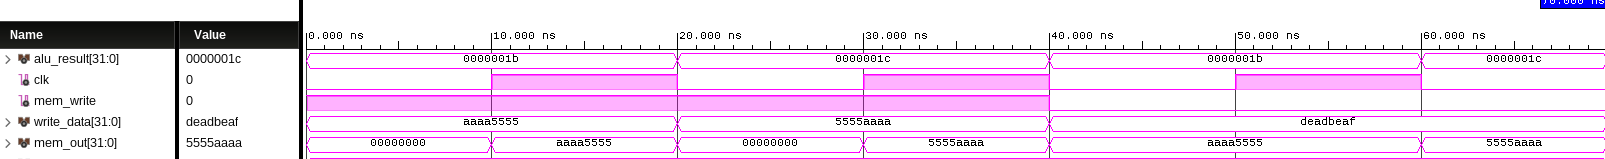
\includegraphics[width=\textwidth]{img/memory_stage_behav}
        \caption{Memory Stage Behavioural Waveform}
        \label{fig:mem_behav}
    \end{figure}
    \begin{figure}[h!]
        \centering
        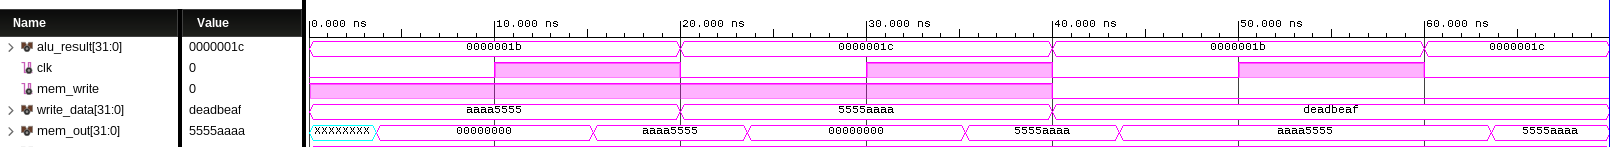
\includegraphics[width=\textwidth]{img/memory_stage_synth}
        \caption{Memory Stage Post-Synthesis Timing Waveform}
        \label{fig:mem_synth}
    \end{figure}
    \begin{figure}[h!]
        \centering
        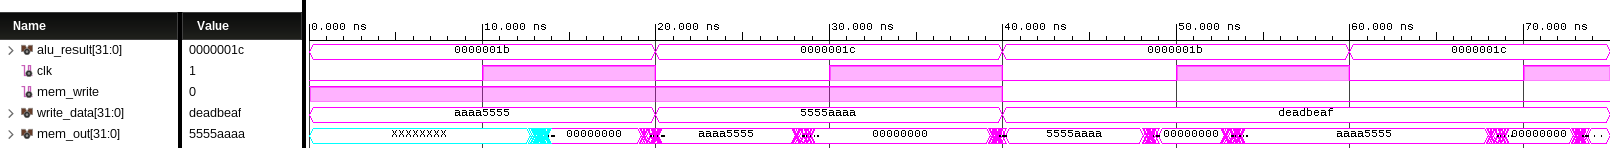
\includegraphics[width=\textwidth]{img/memory_stage_impl}
        \caption{Memory Stage Post-Implementation Timing Waveform}
        \label{fig:mem_impl}
    \end{figure}
    
    Figures \ref{fig:mem_behav} \ref{fig:mem_synth} and \ref{fig:mem_impl}
    show the testcases described in Table \ref{tab:mem}. Looking at the two
    timing simulations in Figures \ref{fig:mem_synth} and \ref{fig:mem_impl},
    we cna see that the shortened clock period of 20ns is still long enough
    to provide ample setup time for the writeback stage.

    \subsection*{Writeback Stage}

	To test the writeback stage, the two different possible testcases need
	to be run. The writeback stage will select between the ALU result and the
	read memory output. A waveform was generated to show the proper
	functionality of the writeback stage.
	
	\begin{figure}[h!]
        \centering
        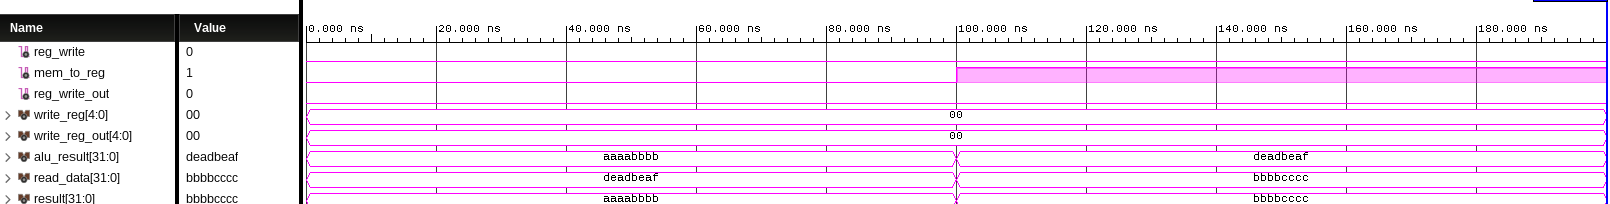
\includegraphics[width=\textwidth]{img/writeback_stage_behav}
        \caption{Writeback Stage Behavioural Waveform}
        \label{fig:writeback}
    \end{figure}
    
    Figure \ref{fig:writeback} will show that the mux selection for the
    writeback stage will properly select from the two input signals:
    \code{alu\_result} and \code{mem\_result}.

	\pagebreak

    \section*{Conclusion}
    
    This laboratory exercise implemented the memory stage and the writeback
    stage. The memory stage wraps the data memory by passing the address
    from the ALU result into the data memory.
    No special handling is needed for any of the addresses in data memory.
    The writeback stage will simply select between the memory read output
    and the ALU result. The generated waveforms from the memory stage and 
    the writeback stage show that the implementation works properly.

    \pagebreak

    \section*{Demo results}
    
    \subsection*{Part1}
    \begin{figure}[h!]
        \centering
        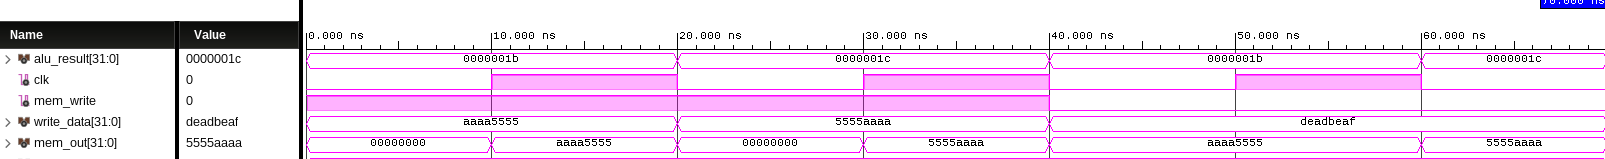
\includegraphics[width=\textwidth]{img/memory_stage_behav}
        \caption{Behavioural simulation of Memory Stage}
        %! suppress = FigureNotReferenced
        \label{fig:demo1}
	\end{figure}
    \begin{figure}[h!]
        \centering
        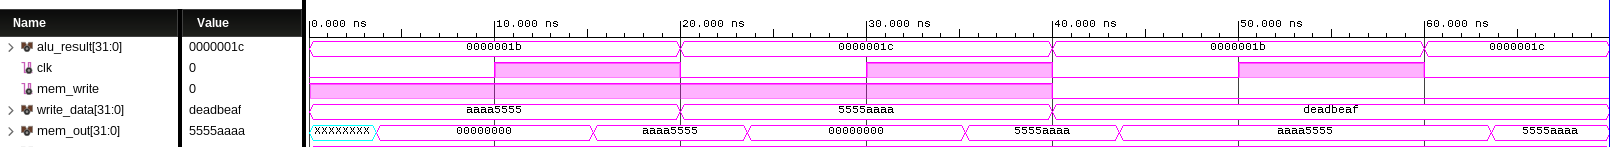
\includegraphics[width=\textwidth]{img/memory_stage_synth}
        \caption{Post-synthesis timing simulation of Memory Stage}
        %! suppress = FigureNotReferenced
        \label{fig:demo1}
	\end{figure}
    \begin{figure}[h!]
        \centering
        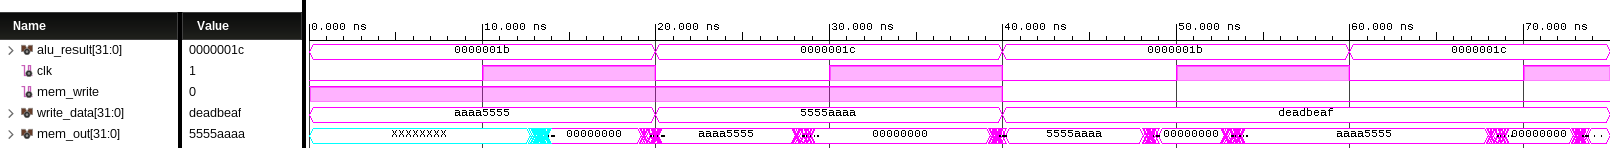
\includegraphics[width=\textwidth]{img/memory_stage_impl}
        \caption{Post-implementation timing simulation of Memory Stage}
        %! suppress = FigureNotReferenced
        \label{fig:demo1}
	\end{figure}
    \subsection*{Part2}
    \begin{figure}[h!]
        \centering
        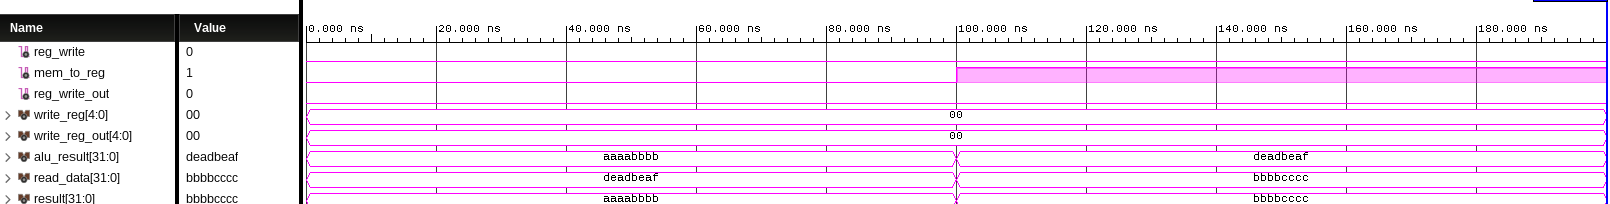
\includegraphics[width=\textwidth]{img/writeback_stage_behav}
        \caption{Behavioural simulation of Writeback Stage}
        %! suppress = FigureNotReferenced
        \label{fig:demo1}
	\end{figure}
    \begin{figure}[h!]
        \centering
        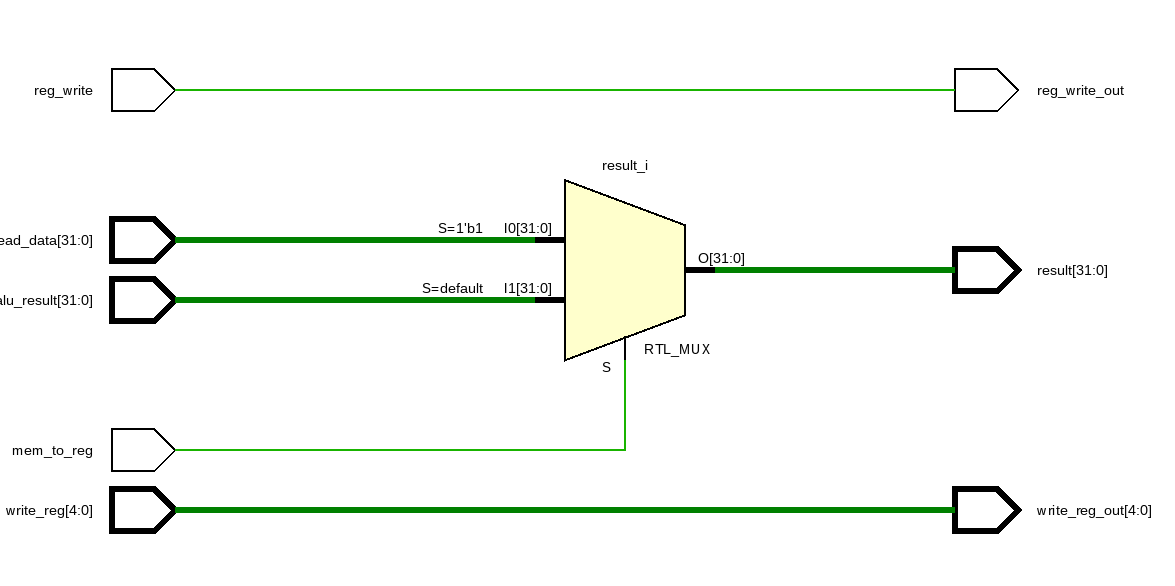
\includegraphics[width=\textwidth]{img/writeback_stage_schem}
        \caption{Writeback Stage RTL schematic}
        %! suppress = FigureNotReferenced
        \label{fig:demo1}
	\end{figure}
    

\end{document}